\documentclass[conference]{IEEEtran}
\IEEEoverridecommandlockouts

% Margin safety adjustment for PDF eXpress / conference preflight.
% Shifts the text area down by 0.05 in while preserving the bottom margin.
\addtolength{\topmargin}{0.05in}
\addtolength{\textheight}{-0.05in}

\usepackage{cite}
\usepackage{amsmath,amssymb,amsfonts}
\usepackage{graphicx}
\usepackage{textcomp}
\usepackage{xcolor}
\usepackage{booktabs}
\usepackage{array}
\usepackage{url}
\usepackage{tikz}
\usetikzlibrary{arrows.meta,positioning,shapes.geometric}

\graphicspath{{figures/}{./}}

\newcommand{\figplaceholder}[2]{%
\fbox{\begin{minipage}[c][#1][c]{0.94\columnwidth}
\centering\small #2
\end{minipage}}}

\newcommand{\widefigplaceholder}[2]{%
\fbox{\begin{minipage}[c][#1][c]{0.94\textwidth}
\centering\small #2
\end{minipage}}}

\def\BibTeX{{\rm B\kern-.05em{\sc i\kern-.025em b}\kern-.08em
    T\kern-.1667em\lower.7ex\hbox{E}\kern-.125emX}}

\begin{document}

\title{Channel-Aware Backdoor Attacks Against Federated Infostealer Malware Classification Using Dynamic API-Call and Network Representations}

\author{
\IEEEauthorblockN{1\textsuperscript{st} Mochamad Asryl Aziz}
\IEEEauthorblockA{ 
\textit{BPS-Statistics Indonesia}\\
\textit{Bantaeng Regency}\\
Bantaeng, South Sulawesi, Indonesia\\
mochamadasryl93@gmail.com
}
\and
\IEEEauthorblockN{2\textsuperscript{nd} Moh. Jabir Mubarok}
\IEEEauthorblockA{
	\textit{Department of Electrical Engineering}\\
	\textit{Faculty of Intelligent Electrical and}\\
	\textit{Informatics Technology}\\
	\textit{Institut Teknologi Sepuluh Nopember}\\
	Surabaya, Indonesia\\
	jabirmubarok@gmail.com
}
\and
\IEEEauthorblockN{3\textsuperscript{rd} Eka Fitria}
\IEEEauthorblockA{
\textit{Department of Informatics}\\
\textit{Faculty of Mathematics}\\
\textit{and Natural Science}\\
\textit{Universitas Syiah Kuala}\\
Banda Aceh, Indonesia\\
ekafitria2@mhs.usk.ac.id
}
}

\maketitle

\begin{abstract}
	Federated learning (FL) facilitates collaborative malware model training while preserving the privacy of local data. However, its dependence on updates submitted by participating clients exposes the system to backdoor poisoning attacks.
	This paper evaluates channel-aware backdoor attacks against federated infostealer malware family classification using dynamic API-call and network representations. We use five Windows infostealer families, 100 samples each, and compare RGB-stack and opacity-blend representations across SmallCNN, MobileNetV2 and ResNet18. RGB-stack is used because it separates the channels explicitly, and ResNet18 is its strongest backbone at 78.67\% accuracy and 78.84\% macro-F1. Under five-client FedAvg the clean baseline reaches 82.67\% accuracy and 82.55\% macro-F1 across three seeds. We then inject targeted AgentTesla-to-FormBook triggers into the red/API, green/network, blue/fusion and full-RGB channels. 
	The blue/fusion and full-RGB triggers both reach 100\% attack success rate (ASR) across three seeds while keeping clean performance close to the baseline, and in seven of the eight trigger controls the target rate is identical with and without the trigger, so the ASR cannot be attributed to the trigger pattern itself. The novelty is to treat the channels of the representation as the attack surface: a trigger confined to the fusion channel alone is as effective as one spanning all three, even though that channel is derived from the other two. Multi-Krum does not mitigate this in a graded way; for each trigger it leaves the backdoor fully effective on one of the three seeds, and on full RGB it lowers clean accuracy from 84.00\% to 76.00\%. Channel-aware backdoors are therefore a serious threat to federated malware classifiers in this controlled IID setting, and motivate representation-aware defenses.
\end{abstract}

\begin{IEEEkeywords}
	Federated learning, malware classification, backdoor attack, robust aggregation, dynamic malware representation.
\end{IEEEkeywords}

\section{Introduction}

Infostealer malware targets authentication artifacts such as credentials, browser data and session cookies, which can enable account compromise and unauthorized access \cite{thomas2017stolencredentials,franken2018cookiejar,nayak2024browserextensions}. Classifying infostealer families therefore matters for threat intelligence, triage and incident response.

Dynamic analysis captures runtime behavior beyond static file properties: API-call sequences represent host-level execution \cite{wu2025mines} and network artifacts capture communication patterns \cite{davis2024traffic}, and both can be encoded into CNN-compatible images \cite{xuan2024rgbfusion}.



Federated learning (FL) lets participants train such a classifier together without moving raw data to a central server \cite{nobakht2024simfed}, but its reliance on client-submitted updates lets a malicious client inject backdoor behavior \cite{ren2024shadow}.

Most FL backdoor work targets general image or model-level poisoning rather than channel-specific behavior in malware representations \cite{ren2024shadow}. This matters because an RGB-stack representation places API-call, network and fused information in separate channels \cite{xuan2024rgbfusion}, so a trigger in one channel need not behave like a trigger in another, and colour-space triggers are known to be effective in image-based poisoning \cite{jiang2023color}. That behavior remains underexplored on dynamic API-call and network representations, and this paper investigates it in federated infostealer malware classification.

The main contributions of this paper are as follows:
\begin{itemize}
    \item We construct dynamic API-call and network representations from Cuckoo Sandbox reports of five infostealer families.
    \item We select the main representation--backbone pair by comparing RGB-stack and opacity blend with SmallCNN, MobileNetV2, and ResNet18.
    \item We evaluate channel-aware backdoor attacks in FL using red/API, green/network, blue/fusion, and full-RGB triggers, with trigger-control and Multi-Krum defense analysis.
\end{itemize}

\section{Related Work}

\subsection{Dynamic Malware Representation}

Malware classification can use static, dynamic, or hybrid representations, while dynamic analysis captures runtime behavior such as API calls, file and registry operations, process activity, and network traces \cite{ma2025api}. The API-call \cite{wu2025mines}, network \cite{davis2024traffic}, and RGB-fusion \cite{xuan2024rgbfusion} work introduced in Section~I underpins the representations used here.

\subsection{Federated Learning for Malware Classification}

Federated learning (FL) allows distributed clients to collaboratively train a global model without sharing their raw local data \cite{mcmahan2017fedavg}. This setting is suitable for malware classification because security data may be distributed across organizations or sandbox environments \cite{nobakht2024simfed}. However, FL remains vulnerable because the server depends on client-submitted updates and has limited visibility into local training data \cite{ren2024shadow}.

\subsection{Backdoor Attacks and Robust Aggregation}

Backdoor attacks allow malicious FL participants to implant hidden target behavior while preserving clean-input performance \cite{bagdasaryan2020backdoor}. In malware classification, this may cause a triggered source family to be misclassified as an attacker-specified target family \cite{ren2024shadow}. Robust aggregation methods such as Krum and Multi-Krum identify reliable client updates by comparing their distances to other updates \cite{blanchard2017krum}, while coordinate-wise median and trimmed mean limit the influence of extreme update values \cite{yin2018byzantine}. However, recent defense work shows that robust aggregation may still be insufficient against stealthy backdoor objectives \cite{wang2024rope}. Backdoors have also been studied on malware classifiers directly, through explanation-guided feature-space triggers \cite{severi2021explanation} and family-selective triggers \cite{yang2023jigsaw}. Both target static features of a centralized model; we attack a federated one through the channels of a dynamic-behavior image.

\section{Methodology}
Figure~\ref{fig:methodology} shows the overall workflow. The subsections below follow its blocks in order: dataset creation, representation construction, model selection, the federated setup, the threat model and channel-aware trigger, and the defenses and trigger control. Section~IV then reports the results.

\begin{figure}[h]
	\centering
	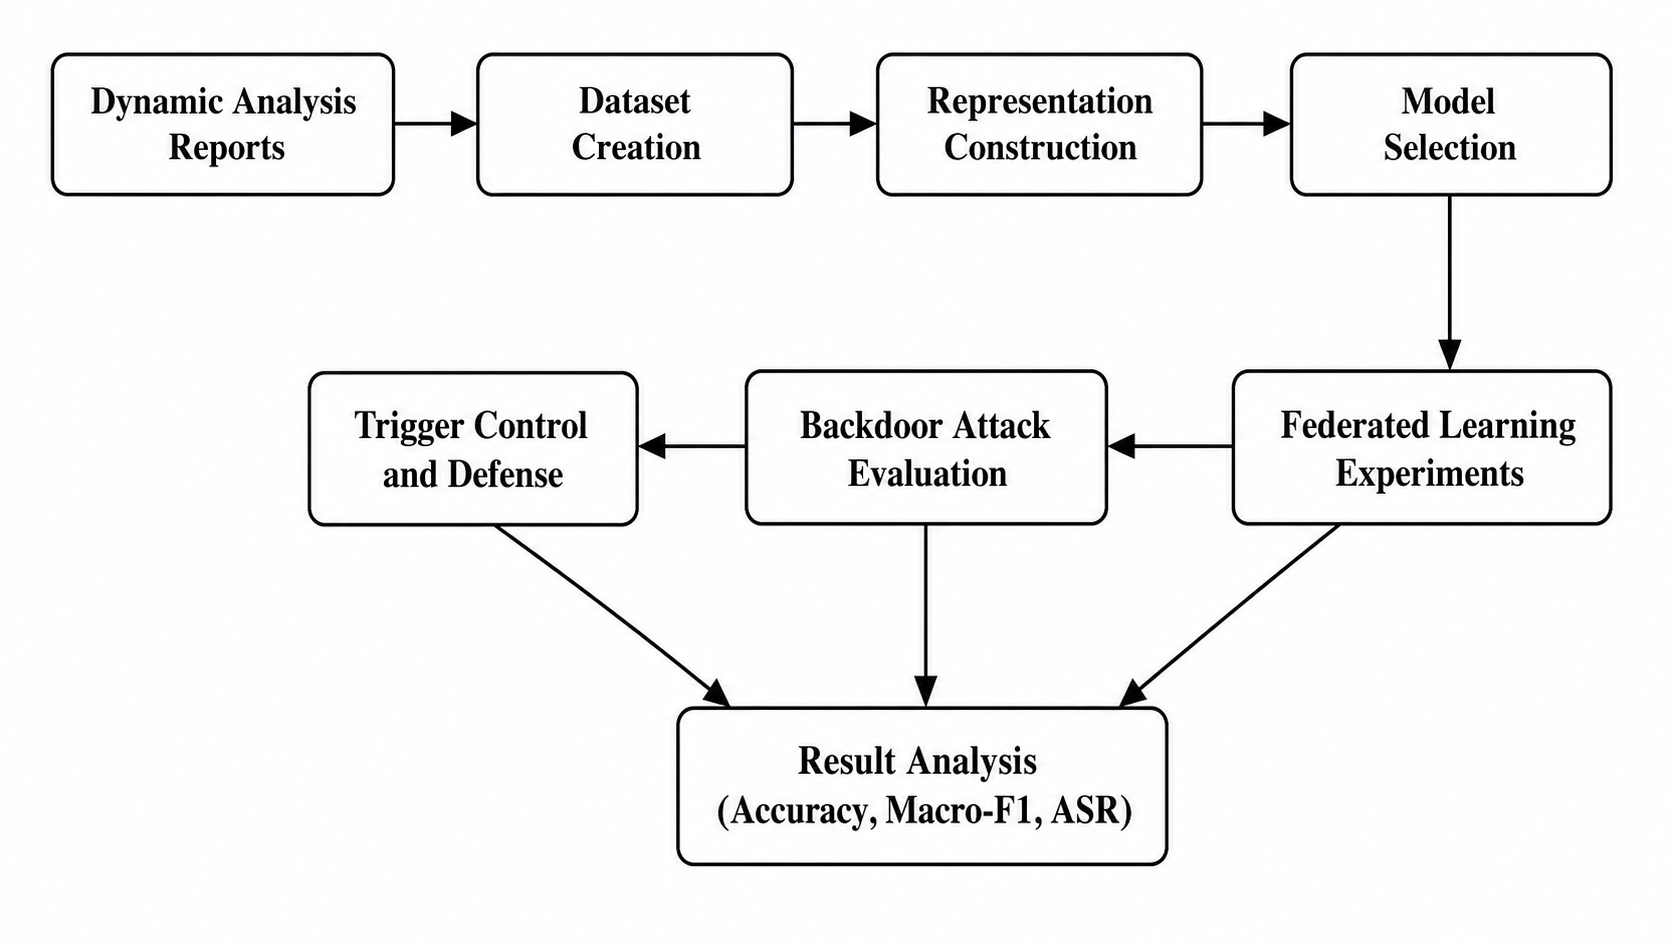
\includegraphics[width=\columnwidth]{method.png}
	\caption{Overall research workflow of the proposed study.}
	\label{fig:methodology}
\end{figure}

\subsection{Dataset Creation}

The dataset is built from Cuckoo Sandbox reports for five Windows infostealer families: AgentTesla, FormBook, SalatStealer, StealC and Vidar. The sandbox runs each sample in isolation and yields the API-call traces and network artifacts used here \cite{pektas2018api,wu2025mines}.

API-call events are converted into a $16 \times 16$ category-by-time tile by normalizing the execution timeline, mapping API names into predefined behavior categories, and counting category occurrences over fixed time intervals \cite{chen2024ctimd}. Network artifacts are reconstructed from packet captures using flow-level identifiers. To reduce sample-level leakage, only the session with the largest payload is selected for each malware sample, then truncated or padded and reshaped into a $28 \times 28$ network tile \cite{davis2024traffic}. Figure~\ref{fig:dataset} illustrates this pipeline, and Table~\ref{tab:dataset} summarizes the resulting dataset.

Tiles are aligned per sample and recorded in a manifest organized by family, which supports stratified splitting and reproducibility \cite{vasan2020imcec}. At training time the 8-bit images are normalized to $[-1,1]$.

With 100 samples per family the dataset holds 500 representations, split 70\%--15\%--15\% into training, validation and test partitions, stratified by family.

\begin{table}[h]
	\caption{Dataset Summary and Stratified Split}
	\label{tab:dataset}
	\centering
	\begin{tabular}{lcccc}
		\toprule
		\textbf{Family} & \textbf{Total} & \textbf{Train} & \textbf{Val.} & \textbf{Test} \\
		\midrule
		AgentTesla   & 100 & 70 & 15 & 15 \\
		FormBook     & 100 & 70 & 15 & 15 \\
		SalatStealer & 100 & 70 & 15 & 15 \\
		StealC       & 100 & 70 & 15 & 15 \\
		Vidar        & 100 & 70 & 15 & 15 \\
		\midrule
		Total        & 500 & 350 & 75 & 75 \\
		\bottomrule
	\end{tabular}
\end{table}

\subsection{Dynamic API Call and Network Representations}

We evaluate two representation strategies: RGB-stack and opacity blend. 
Both representations transform dynamic API-call and network artifacts into CNN-compatible images, following prior image-based malware classification studies \cite{vasan2020imcec}. 

In RGB-stack the API and network tiles are grayscaled, min--max normalized per image and resized to $128 \times 128$; red carries API-call behavior, green network behavior \cite{xuan2024rgbfusion}, and blue is the edge map of their average, $B = \mathrm{FindEdges}((R+G)/2)$, with $\mathrm{FindEdges}$ a $3 \times 3$ edge-detection convolution. Blue is thus a deterministic function of the other two channels, adds no independent information, and is by far the emptiest: 54.5\% of its pixels are exactly zero. Opacity blend instead modulates the colour API image by a network-derived texture, so none of its channels corresponds to a single source; RGB-stack is used here because only it separates the sources by channel.

Figure~\ref{fig:sample} shows representative processed malware representations used in this study.

\begin{figure}[t]
	\centering
	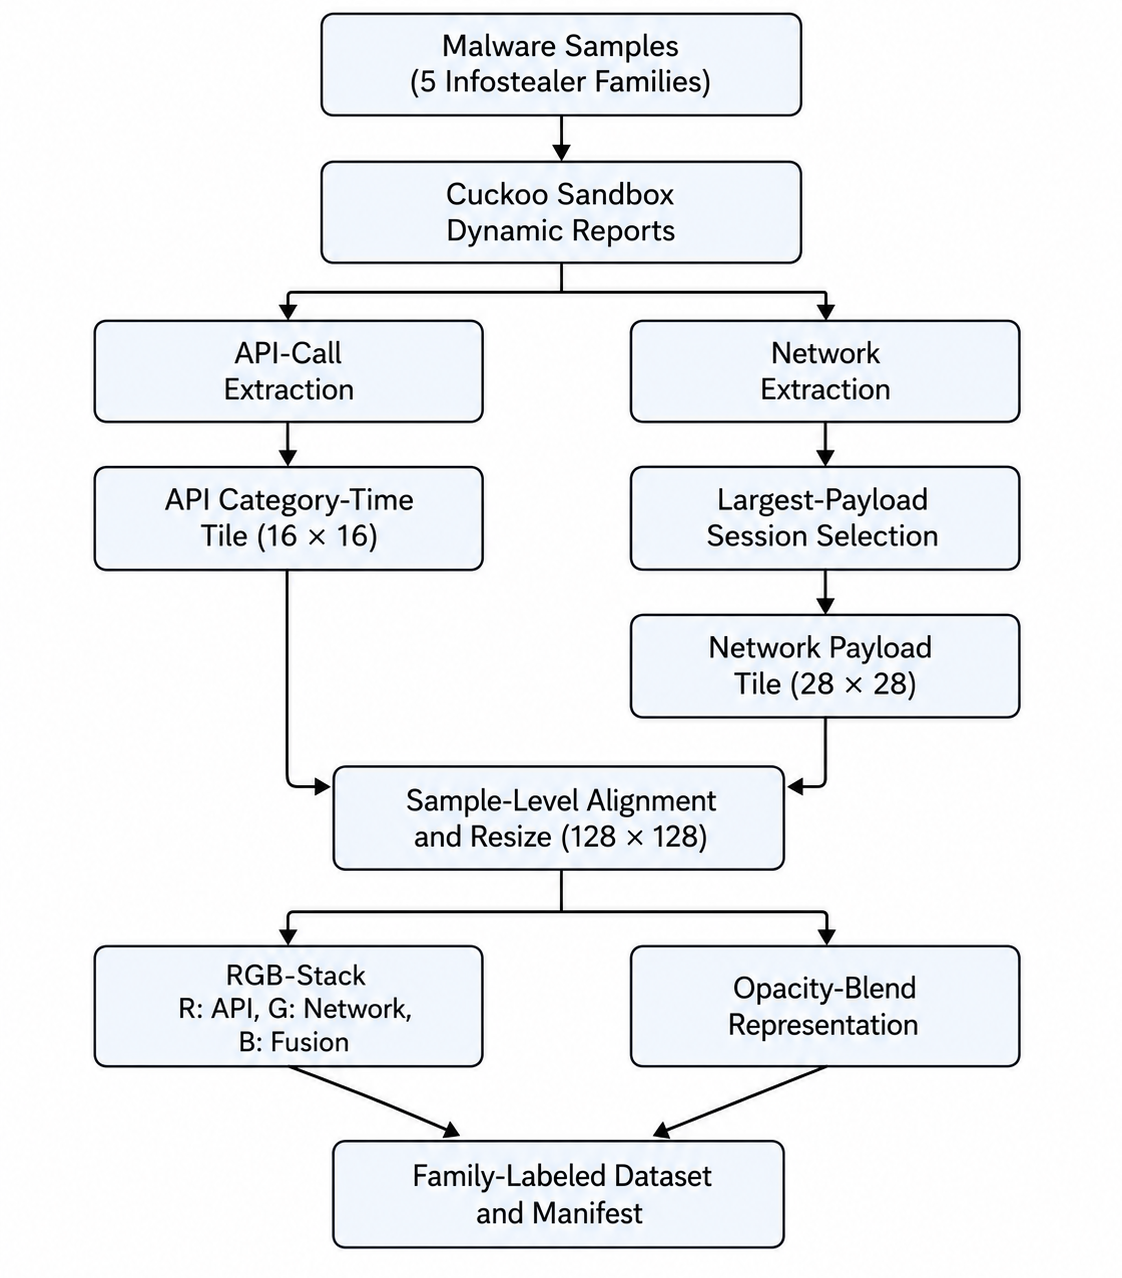
\includegraphics[width=0.70\columnwidth]{dataset.png}
	\caption{Dataset creation pipeline from dynamic analysis reports to dynamic API-call and network representations.}
	\label{fig:dataset}
\end{figure}

\begin{figure}[t]
	\centering
	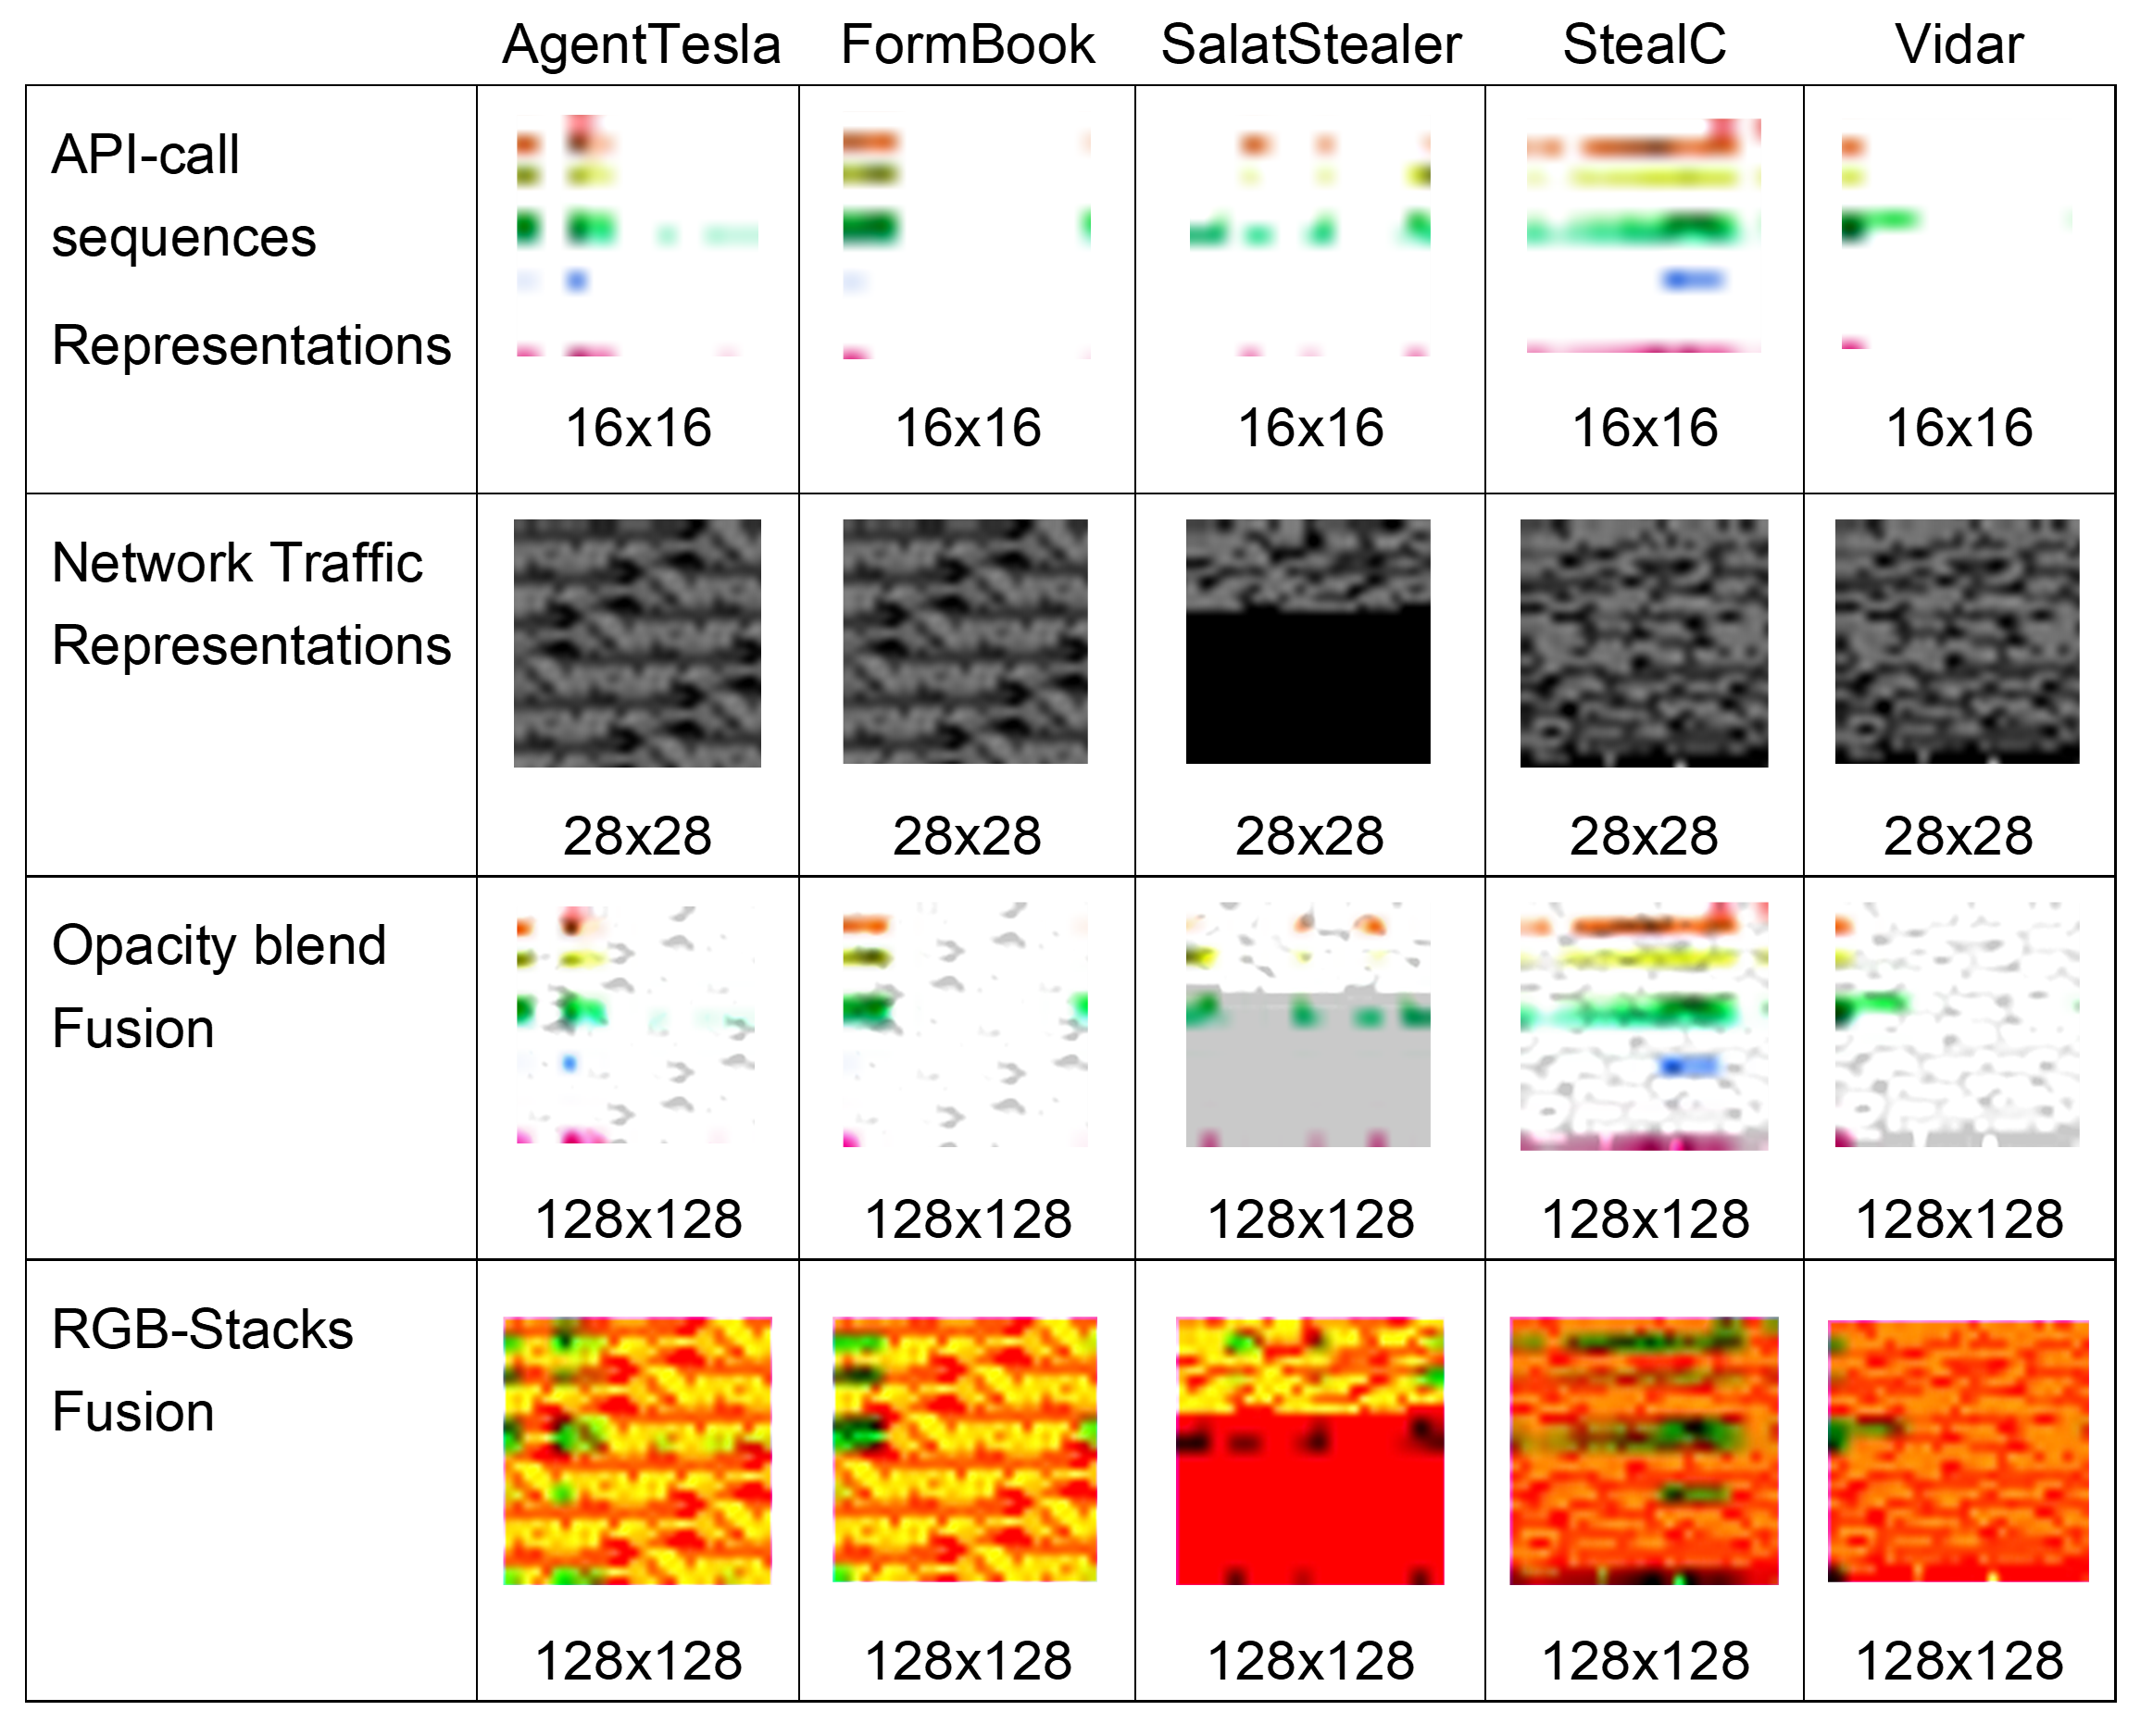
\includegraphics[width=0.70\columnwidth]{malware.png}
	\caption{Representative processed malware representations generated from dynamic API-call and network packet artifacts. Rows illustrate different representation types, while columns correspond to the five infostealer families.}
	\label{fig:sample}
\end{figure}

\subsection{Model Selection}

Before the FL and backdoor experiments, we evaluate RGB-stack and opacity blend with three CNN backbones: SmallCNN, MobileNetV2, and ResNet18. 
SmallCNN is a three-block network (32/64/128 channels, Conv $3 \times 3$ + BN + ReLU, max-pooling after the first two blocks, adaptive average pooling, then a linear layer to five classes); MobileNetV2 and ResNet18 are the efficient and residual references \cite{zhang2025imcmk,sandler2018mobilenetv2,he2016resnet}, all trained from scratch. The two representations use different split files, so Table~\ref{tab:backbone} is not a paired comparison across representations: RGB-stack is chosen because channel separation is required here, and macro-F1 only selects the backbone within it.

\subsection{Federated Learning Server and Clients}

The selected representation--backbone pair is trained in a simulated FL setting with one central server and five clients, shown in Fig.~\ref{fig:federated}. Each client holds 70 images, 14 per family, so the partition is balanced and IID. 
Clients train locally; the server distributes the global model and aggregates updates without seeing raw data \cite{nobakht2024simfed}. 

In each communication round, clients send their updated parameters to the server, which aggregates them with FedAvg:

\begin{equation}
	w^{t+1} = \sum_{k=1}^{K} \frac{n_k}{n} w_k^{t+1},
\end{equation}
where $w^{t}$ is the global model at round $t$, $w_k^{t+1}$ the model trained locally by client $k$, $n_k$ the number of samples on client $k$, $n$ the total, and $K=5$ the number of clients. The figure writes the model as $\omega$.

In the attack setting, one of the five clients acts as a malicious client that injects poisoned local updates into the FL process \cite{fang2023vulnerability}.

\begin{figure}[h]
	\centering
	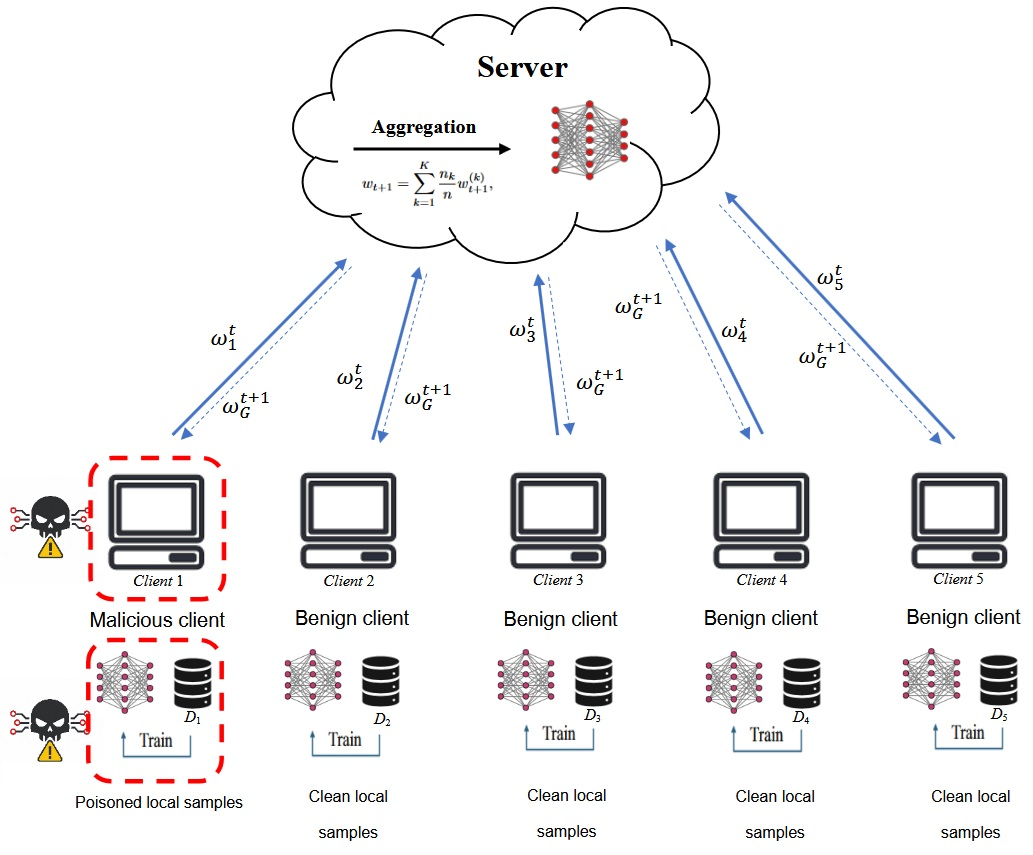
\includegraphics[width=0.60\columnwidth]{federated.jpg}
	\caption{Federated learning architecture used in this study, consisting of one central server and five clients. One client is malicious in the backdoor attack setting.}
	\label{fig:federated}
\end{figure}

\subsection{Threat Model and Channel-Aware Trigger}

We assume a targeted backdoor with one malicious client \cite{ren2024shadow}: it inserts a square image-level trigger into AgentTesla training images and relabels them FormBook \cite{jiang2023color}. AgentTesla is a prominent malware-as-a-service family \cite{bhanot2025agenttesla} and the two are behaviorally related, so the pair is a realistic same-category target. The poison rate is 20\% of the attacker's 14 AgentTesla training images, i.e. two images per round, resampled every round. The trigger is a white $12 \times 12$ square written bottom-right after normalization, so $T(\cdot)$ writes into one channel for red, green and blue and into all three for full RGB. The malicious client is client 0 and participates in every round; its capability is pure data poisoning, with no update scaling and no model replacement, so \cite{bagdasaryan2020backdoor} is background rather than the attack used here.

Because RGB-stack preserves channel-level semantics, four trigger settings are evaluated: red/API, green/network, blue/fusion and full RGB. ASR is the fraction of triggered source-class samples classified as the target class \cite{liu2024persistent}:
\begin{equation}
	\mathrm{ASR} =
	\frac{
		|\{x_i : y_i = y_s,\; f(T(x_i)) = y_t\}|
	}{
		|\{x_i : y_i = y_s\}|
	},
\end{equation}
where $y_s$ is the source label, $y_t$ is the target label, $T(\cdot)$ denotes the trigger insertion function, and $f(\cdot)$ denotes the trained classifier.

\subsection{Defense}

Multi-Krum is the primary defense, taken as a standard robust-aggregation baseline: it scores client updates by their distances to other updates and aggregates those with the lowest scores \cite{blanchard2017krum}. Let $w_k^{t+1}$ denote the local model update submitted by client $k$ at communication round $t+1$. The pairwise distance between two client updates is computed as:
\begin{equation}
	d_{k,j} =
	\left\|
	w_k^{t+1} - w_j^{t+1}
	\right\|_2^2,
\end{equation}

For each client $k$, the Multi-Krum score is defined as:
\begin{equation}
	s_k =
	\sum_{j \in \mathcal{N}_k}
	d_{k,j},
\end{equation}

where $\mathcal{N}_k$ denotes the set of closest neighboring updates to client $k$. 
Here $K=5$ and $f=1$, so the score uses the two nearest updates and the $|\mathcal{S}|=2$ lowest-scoring of five are averaged. $L_2$-norm clipping, coordinate-wise median and trimmed mean are screened alongside it \cite{yin2018byzantine}. As a control, the same triggers are applied at test time to the clean FL model, which never saw poisoned data, so its target predictions are baseline family confusion.

The server keeps the subset $\mathcal{S}$ of lowest-scoring updates and forms the defended global model. All clients hold 70 images, so the sample-weighted average reduces to:
\begin{equation}
	w^{t+1} =
	\frac{1}{|\mathcal{S}|}
	\sum_{k \in \mathcal{S}}
	w_k^{t+1}.
\end{equation}

\subsection{Experimental Setup}

Dynamic analysis and model training run on the separate environments listed in Table~\ref{tab:environment}.

\begin{table}[h]
	\caption{Experimental Environment}
	\label{tab:environment}
	\footnotesize
	\centering
	\setlength{\tabcolsep}{4pt}
	\begin{tabular}{ll}
		\toprule
		\textbf{Component} & \textbf{Specification} \\
		\midrule
		Dynamic analysis & Cuckoo Sandbox on Ubuntu \\
		Training environment & Windows, Python / Anaconda \\
		Framework & PyTorch with CUDA 12.8 \\
		GPU & NVIDIA GeForce RTX 3080, 12 GB VRAM \\
		\bottomrule
	\end{tabular}
\end{table}

\subsection{Training Configuration}

All representations are resized to $128 \times 128$ pixels. The selected ResNet18 has five output classes and is trained with cross-entropy loss. 
Training uses a batch size of 16, learning and weight decay rates of $10^{-4}$, 50 FL rounds, and two local epochs per round. One deviation must be stated: the seed-42 clean baseline in Table~\ref{tab:main} and the seed-42 trigger controls come from a 30-round, one-local-epoch run. Re-training it under the common budget gives 0.7867 accuracy, 0.7869 macro-F1 and a control rate of 6/15 rather than 4/15, so the reported run sets a higher bar for the clean-performance claim and a lower one for the trigger-control argument. No ASR result is affected; every backdoor and defense run uses the common budget. ResNet18 is trained from scratch with AdamW, and the reported FL model is the final-round global model, with no best-validation selection; the validation split is not used in the backdoor runs, so the per-round curves in Figs.~\ref{fig:f1_round}--\ref{fig:all_settings_round} are test-set curves. Clean accuracy, macro-F1, and ASR are reported as primary metrics, and the main experiments are repeated over three seeds: 42, 123, and 2026.

\section{Results and Discussion}
\subsection{Backbone Selection Results}
Table~\ref{tab:backbone} shows the backbone selection results using seed 42. 
Among the RGB-stack backbones ResNet18 is the strongest, at 78.67\% accuracy and 78.84\% macro-F1, and is used for all later experiments; the opacity-blend rows come from a different split and are listed for reference only.

\begin{table}[h]
\caption{Backbone Selection Study Using Seed 42}
\label{tab:backbone}
\centering
\footnotesize
\begin{tabular}{llcc}
\toprule
\textbf{Representation} & \textbf{Backbone} & \textbf{Acc.} & \textbf{Macro-F1} \\
\midrule
Opacity blend & SmallCNN & 0.5333 & 0.5298 \\
Opacity blend & MobileNetV2 & 0.6933 & 0.6903 \\
Opacity blend & ResNet18 & 0.7733 & 0.7730 \\
RGB-stack & SmallCNN & 0.5200 & 0.5144 \\
RGB-stack & MobileNetV2 & 0.7200 & 0.7200 \\
\textbf{RGB-stack} & \textbf{ResNet18} & \textbf{0.7867} & \textbf{0.7884} \\
\bottomrule
\end{tabular}
\end{table}

\subsection{Channel-Aware Backdoor Sweep}

Table~\ref{tab:sweep} shows that blue/fusion and full-RGB triggers achieve 100\% ASR, while red/API and green/network triggers do not, and the blue/fusion trigger reaches perfect ASR without modifying all RGB channels. The difference is categorical. Pooled over the triggered samples, blue/fusion and full RGB differ from their trigger controls at Fisher exact $p = 3.5 \times 10^{-19}$ and $p = 2.6 \times 10^{-18}$, and blue differs from red and green at $p = 4.0 \times 10^{-8}$, whereas red and green are indistinguishable from their own controls (both $p = 1$, 5/15 against 4/15, seed 42 only). Pooling is legitimate because the split is re-drawn per seed. The ordering follows the intensity of the clean images: over all 500 images the mean value inside the trigger region is 241.7 in R, 81.5 in G and 10.2 in B, and 37.7\% of red trigger-region pixels are already at least 254, where the trigger changes nothing. Contrast explains red's failure but not green's, whose contrast is 207. Since blue is a deterministic edge map of the other two, its effectiveness cannot come from information they lack; what distinguishes it is that it is almost empty, so the trigger is the only strong response there.

\begin{table}[h]
\caption{Channel-Aware Backdoor Sweep Using Seed 42}
\label{tab:sweep}
\centering
\footnotesize
\begin{tabular}{lccc}
\toprule
\textbf{Trigger} & \textbf{Clean Acc.} & \textbf{Macro-F1} & \textbf{ASR} \\
\midrule
Red/API & 0.8533 & 0.8524 & 0.3333 \\
Green/network & 0.8400 & 0.8419 & 0.3333 \\
Blue/fusion & 0.8400 & 0.8395 & 1.0000 \\
Full RGB & 0.8400 & 0.8401 & 1.0000\\
\bottomrule
\end{tabular}
\end{table}

\subsection{Defense Screening}

Four defenses are screened on a single seed before the multi-seed evaluation. Screening every defense across every seed would multiply the training budget by the number of seeds for candidates that may not be worth carrying forward, and all runs share one GPU, so the screening narrows the candidates cheaply and only the surviving defense is then evaluated across seeds.

Table~\ref{tab:defense_screening} gives a seed-42 screening against both strongest attacks: clipping, coordinate-wise median and trimmed mean all leave ASR at 1.0000. Only Multi-Krum reduces it, and only under full RGB (1.0000 to 0.4000, clean accuracy 0.8400 to 0.7600), so Multi-Krum is taken to the multi-seed evaluation.

\begin{table}[h]
	\caption{Single-Seed Defense Screening Against Strongest Attacks Using Seed 42}
	\label{tab:defense_screening}
	\centering
	\footnotesize
	\setlength{\tabcolsep}{5pt}
	\begin{tabular}{llccc}
		\toprule
		\textbf{Trigger} & \textbf{Defense} & \textbf{Clean Acc.} & \textbf{Macro-F1} & \textbf{ASR} \\
		\midrule
		Blue/fusion & None & 0.8400 & 0.8395 & 1.0000 \\
		Blue/fusion & Clipping & 0.8533 & 0.8550 & 1.0000 \\
		Blue/fusion & Median & 0.8133 & 0.8120 & 1.0000 \\
		Blue/fusion & Trimmed mean & 0.8267 & 0.8244 & 1.0000 \\
		Blue/fusion & Multi-Krum & 0.8267 & 0.8244 & 1.0000 \\
		\midrule
		Full RGB & None & 0.8400 & 0.8401 & 1.0000 \\
		Full RGB & Clipping & 0.8533 & 0.8550 & 1.0000 \\
		Full RGB & Median & 0.8400 & 0.8388 & 1.0000 \\
		Full RGB & Trimmed mean & 0.8133 & 0.8145 & 1.0000 \\
		Full RGB & Multi-Krum & 0.7600 & 0.7542 & 0.4000 \\
		\bottomrule
	\end{tabular}
\end{table}

\subsection{Multi-Seed Results}

Table~\ref{tab:main} shows that blue/fusion and full-RGB backdoors achieve 100\% ASR across three seeds while maintaining clean performance comparable to the clean FL baseline. 

In the trigger controls the target rate is identical with and without the trigger in 7 of the 8 runs, so what the control measures is the clean model's baseline AgentTesla-to-FormBook confusion rather than any effect of the trigger; the 100\% ASR under poisoning cannot be attributed to the trigger pattern.

\begin{table*}[h]
	\caption{Main Multi-Seed Results Under IID Federated Setting, With Per-Seed Values}
	\label{tab:main}
	\centering
	\footnotesize
	\setlength{\tabcolsep}{5pt}
	\begin{tabular}{llcccc}
		\toprule
		\textbf{Scenario} & \textbf{Channel} & \textbf{Clean Acc.} & \textbf{Macro-F1} & \textbf{ASR / Target Rate} & \textbf{Per seed (42, 123, 2026)} \\
		\midrule
		Clean FL & -- & $0.8267 \pm 0.0134$ & $0.8255 \pm 0.0104$ & -- & -- \\
		Trigger control & Blue/fusion & $0.8267 \pm 0.0134$ & $0.8255 \pm 0.0104$ & $0.1333 \pm 0.1155$ & 4/15, 1/15, 1/15 \\
		Trigger control & Full RGB & $0.8267 \pm 0.0134$ & $0.8255 \pm 0.0104$ & $0.1556 \pm 0.1018$ & 4/15, 1/15, 2/15 \\
		Backdoor, FedAvg & Blue/fusion & $0.8311 \pm 0.0539$ & $0.8320 \pm 0.0539$ & $1.0000 \pm 0.0000$ & 15/15, 15/15, 15/15 \\
		Backdoor, FedAvg & Full RGB & $0.8267 \pm 0.0611$ & $0.8262 \pm 0.0621$ & $1.0000 \pm 0.0000$ & 15/15, 15/15, 15/15 \\
		\midrule
		Backdoor, Multi-Krum & Blue/fusion & $0.8178 \pm 0.0154$ & $0.8184 \pm 0.0135$ & $0.5111 \pm 0.4286$\textsuperscript{\dag} & 15/15, 3/15, 5/15 \\
		Backdoor, Multi-Krum & Full RGB & $0.7956 \pm 0.0407$ & $0.7931 \pm 0.0427$ & $0.6000 \pm 0.3464$\textsuperscript{\dag} & 6/15, 15/15, 6/15 \\
		\bottomrule
	\end{tabular}

	\vspace{2pt}
	\begin{minipage}{\textwidth}
		\footnotesize\raggedright
		\textsuperscript{\dag}Across-seed ASR range $\geq 0.5$: the outcome is bimodal, so the mean describes no individual run and the per-seed counts (out of 15 source samples) should be read instead.
	\end{minipage}
\end{table*}
Figure~\ref{fig:f1_round} shows that the strongest backdoor settings keep clean macro-F1 stable over the rounds, and Fig.~\ref{fig:asr_round} that both attacks increase in ASR and reach 100\%.

\begin{figure}[h]
	\centering
	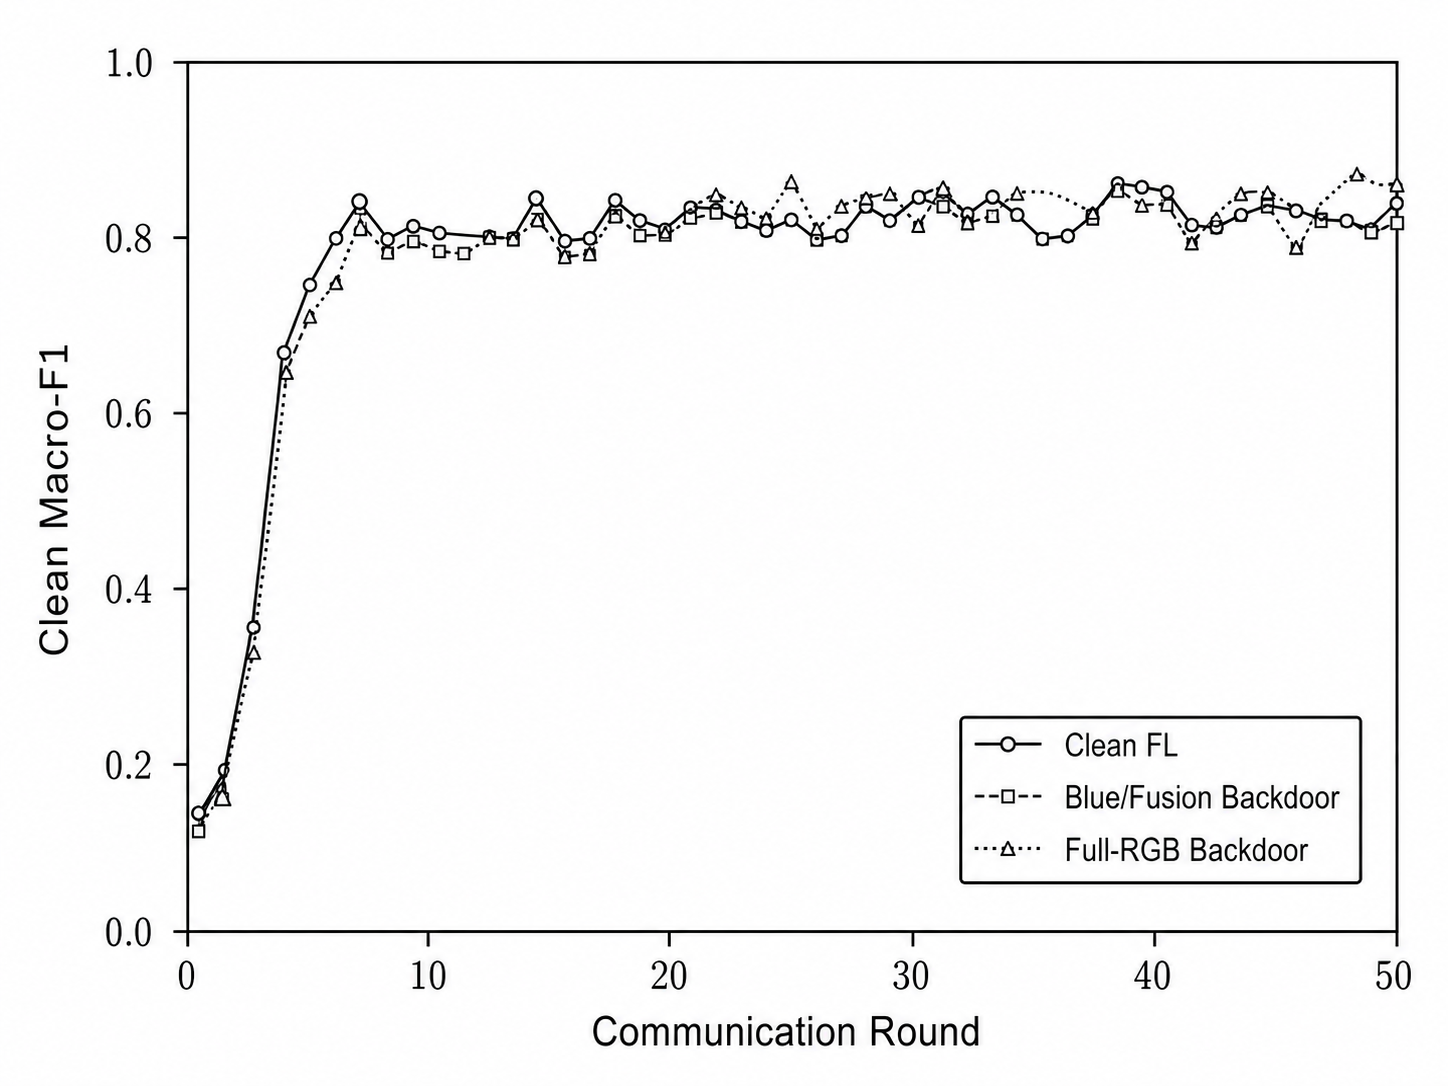
\includegraphics[width=0.65\columnwidth]{clean_per_round.png}
	\caption{Clean macro-F1 over FL communication rounds for the clean FL baseline and the strongest backdoor settings, using seed 42.}
	\label{fig:f1_round}
\end{figure}

\begin{figure}[h]
	\centering
	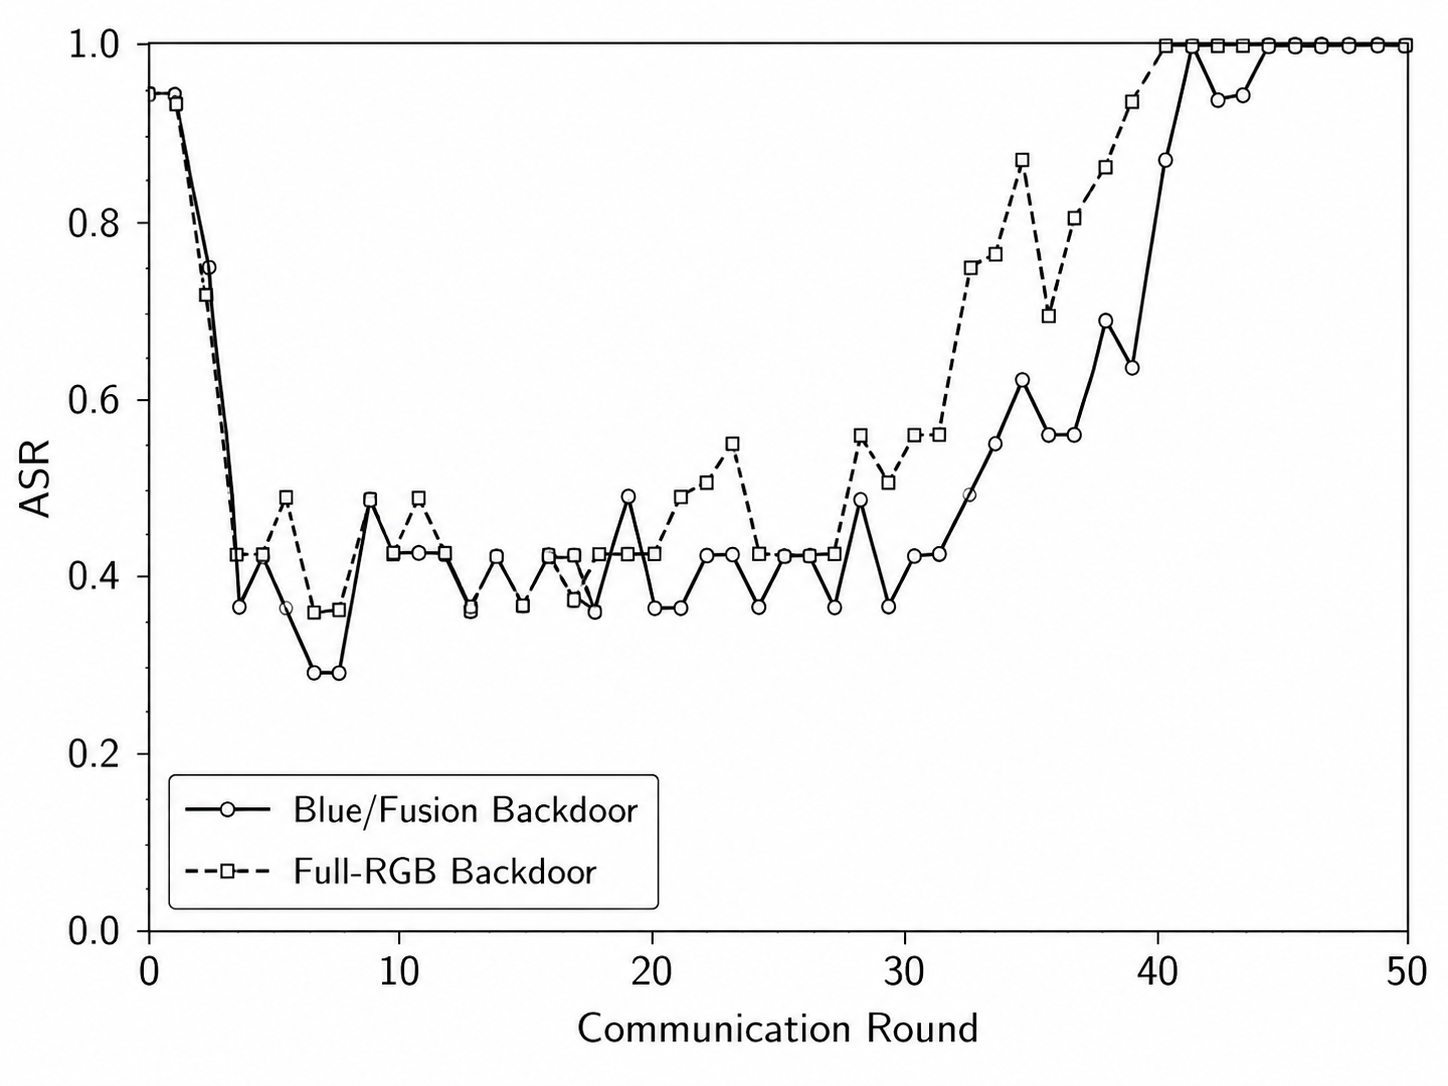
\includegraphics[width=0.65\columnwidth]{asr_per_round.png}
	\caption{Attack success rate (ASR) over FL communication rounds for the strongest blue/fusion and full-RGB backdoor settings, using seed 42.}
	\label{fig:asr_round}
\end{figure}
 The values in the first rounds are not meaningful: the global model is still close to initialization and collapses onto one or two classes, which produces the early spike before clean accuracy rises.
\subsection{Defense Analysis}

The last two rows of Table~\ref{tab:main} report Multi-Krum per seed as well as on average, because the mean is misleading here. For both triggers the across-seed ASR range is at least $0.5$, with nothing in between: on some seeds the backdoor remains fully effective, on the others most of it is suppressed. The outcome is bimodal rather than partial, and $0.5111 \pm 0.4286$ describes no individual run. This also explains the contradiction with the seed-42 screening --- precisely the seed at which blue/fusion + Multi-Krum fails. The outcome tracks how often the poisoned update survives selection: across the six runs the malicious client is retained in 8--50\% of rounds, and that rate correlates with the final ASR ($r = 0.893$, $p = 0.017$, $n = 6$). With $f = 1$ and $|\mathcal{S}| = 2$ of five, the poisoned update is not an outlier in parameter space, so keeping it is close to a coin flip the attacker need only win often enough --- consistent with robust aggregation being insufficient against stealthy objectives \cite{wang2024rope,fang2023vulnerability}. Multi-Krum does reduce ASR against FedAvg ($p = 1.5 \times 10^{-8}$ blue, $p = 9.1 \times 10^{-7}$ full RGB) but costs utility, lowering full-RGB clean accuracy from 0.8400 to 0.7600 on seed 42. No paired clean-performance difference across the three seeds is significant, that drop included (all $p \geq 0.42$, low-powered at $n = 3$).
\begin{figure}[h]
	\centering
	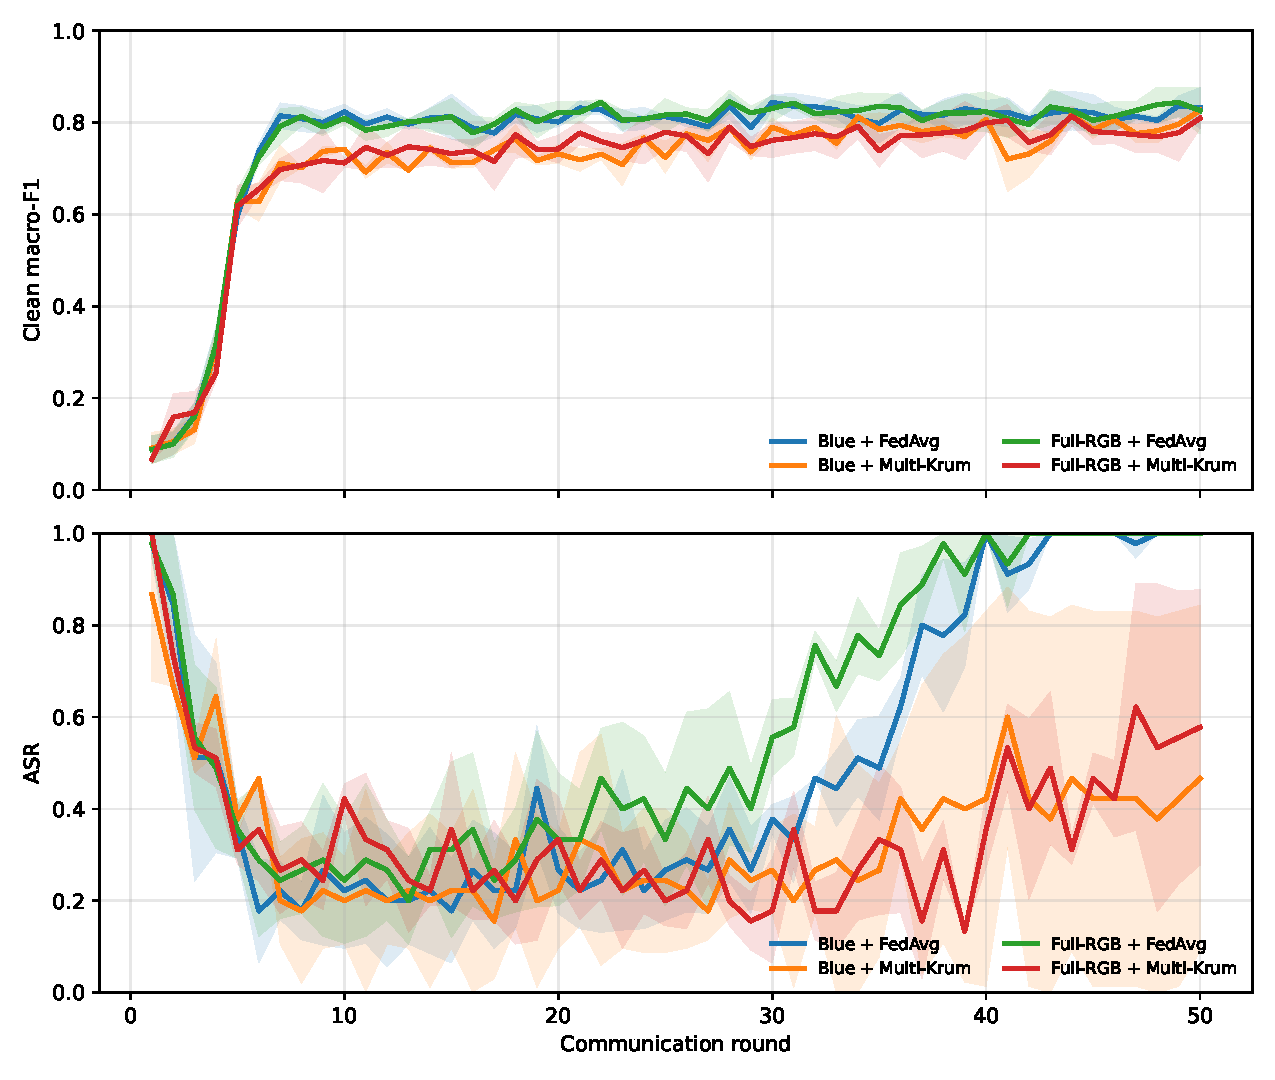
\includegraphics[width=0.38\textwidth]{all_settings_f1_asr_per_round.pdf}
	\caption{Per-round clean macro-F1 and ASR across three random seeds for the blue/fusion and full-RGB backdoor settings under FedAvg and Multi-Krum. Shaded areas denote standard deviation across seeds.}
	\label{fig:all_settings_round}
\end{figure}


Figure~\ref{fig:all_settings_round} shows the per-round clean macro-F1 and ASR across three seeds. 
The clean macro-F1 of the backdoor models remains close to the clean baseline, indicating that the attacks preserve normal classification performance. 
Under FedAvg, both blue/fusion and full-RGB triggers steadily reach 100\% ASR. 
With Multi-Krum, ASR is reduced for both triggers, but the curves remain unstable and show high variation across rounds. 
Consistent with Table~\ref{tab:main}, Multi-Krum does not settle at a stable partial suppression level: for each trigger there is one seed at which it does not suppress the backdoor at all, so it is unreliable as a standalone defense.


\section{Conclusion}

This paper evaluated channel-aware backdoor attacks against federated infostealer malware classification using dynamic API-call and network representations. Blue/fusion and full-RGB triggers reached 100\% ASR across three seeds while keeping clean performance close to the baseline, and in seven of the eight trigger controls the target rate was identical with and without the trigger, so the effect came from poisoning rather than the trigger pattern. Multi-Krum reduced ASR bimodally rather than partially, leaving the backdoor fully effective (15/15) on one of the three seeds for each trigger. Channel-aware backdoors therefore pose a serious threat to federated malware classifiers and motivate representation-aware defenses.

The main limitations are the IID-only partition, a single source--target pair, and three seeds, with the red and green results resting on seed 42 alone. That the blue trigger works because its channel is nearly empty, rather than because of what that channel encodes, is consistent with the measurements but not established; a non-IID partition, a second source--target pair and a contrast-matched trigger are left to future work.

\begin{thebibliography}{00}

\bibitem{thomas2017stolencredentials}
K. Thomas, F. Li, A. Zand, J. Barrett, J. Ranieri, L. Invernizzi,
Y. Markov, O. Comanescu, V. Eranti, A. Moscicki, D. Margolis,
V. Paxson, and E. Bursztein,
``Data breaches, phishing, or malware?: Understanding the risks of stolen credentials,''
in \emph{Proc. ACM SIGSAC Conf. Computer and Communications Security (CCS)},
2017, pp. 1421--1434.

\bibitem{franken2018cookiejar}
G. Franken, T. Van Goethem, and W. Joosen,
``Who left open the cookie jar? A comprehensive evaluation of third-party cookie policies,''
in \emph{Proc. 27th USENIX Security Symposium (USENIX Security)},
2018, pp. 151--168.

\bibitem{nayak2024browserextensions}
A. Nayak, R. Khandelwal, E. Fernandes, and K. Fawaz,
``Experimental security analysis of sensitive data access by browser extensions,''
in \emph{Proc. ACM Web Conf. (WWW)},
2024, pp. 1283--1294.

\bibitem{wu2025mines}
P. Wu, M. Gao, F. Sun, X. Wang, and L. Pan,
``Multi-perspective API call sequence behavior analysis and fusion for malware classification,''
\emph{Computers \& Security}, vol. 148, p. 104177, 2025.

\bibitem{davis2024traffic}
R. E. Davis, J. Xu, and K. Roy,
``Classifying malware traffic using images and deep convolutional neural network,''
\emph{IEEE Access}, vol. 12, pp. 58031--58038, 2024.

\bibitem{xuan2024rgbfusion}
B. Xuan, J. Li, and Y. Song,
``BiTCN-TAEfficientNet malware classification approach based on sequence and RGB fusion,''
\emph{Computers \& Security}, vol. 139, p. 103734, 2024.

\bibitem{nobakht2024simfed}
M. Nobakht, R. Javidan, and A. Pourebrahimi,
``SIM-FED: Secure IoT malware detection model with federated learning,''
\emph{Computers and Electrical Engineering}, vol. 116, p. 109139, 2024.

\bibitem{ren2024shadow}
Q. Ren, Y. Zheng, C. Yang, Y. Li, and J. Ma,
``Shadow backdoor attack: Multi-intensity backdoor attack against federated learning,''
\emph{Computers \& Security}, vol. 139, p. 103740, 2024.

\bibitem{jiang2023color}
W. Jiang, H. Li, G. Xu, and T. Zhang,
``Color backdoor: A robust poisoning attack in color space,''
in \emph{Proc. IEEE/CVF Conf. Computer Vision and Pattern Recognition (CVPR)},
2023, pp. 8133--8142.

\bibitem{ma2025api}
C. Ma, Z. Li, H. Long, A. Bilal, and X. Liu,
``A malware classification method based on directed API call relationships,''
\emph{PLOS ONE}, vol. 20, no. 3, p. e0299706, 2025.

\bibitem{mcmahan2017fedavg}
B. McMahan, E. Moore, D. Ramage, S. Hampson, and B. A. y Arcas,
``Communication-efficient learning of deep networks from decentralized data,''
in \emph{Proc. 20th Int. Conf. Artificial Intelligence and Statistics (AISTATS)},
2017, pp. 1273--1282.

\bibitem{bagdasaryan2020backdoor}
E. Bagdasaryan, A. Veit, Y. Hua, D. Estrin, and V. Shmatikov,
``How to backdoor federated learning,''
in \emph{Proc. 23rd Int. Conf. Artificial Intelligence and Statistics (AISTATS)},
2020, pp. 2938--2948.

\bibitem{blanchard2017krum}
P. Blanchard, E. M. El Mhamdi, R. Guerraoui, and J. Stainer, 
``Machine learning with adversaries: Byzantine tolerant gradient descent,'' 
in \emph{Advances in Neural Information Processing Systems}, vol. 30, 2017.

\bibitem{yin2018byzantine}
D. Yin, Y. Chen, R. Kannan, and P. Bartlett,
``Byzantine-robust distributed learning: Towards optimal statistical rates,''
in \emph{Proc. 35th Int. Conf. Machine Learning (ICML)},
2018, pp. 5650--5659.

\bibitem{wang2024rope}
Y. Wang, D.-H. Zhai, and Y. Xia,
``RoPE: Defending against backdoor attacks in federated learning systems,''
\emph{Knowledge-Based Systems}, vol. 293, p. 111660, 2024.

\bibitem{severi2021explanation}
G. Severi, J. Meyer, S. Coull, and A. Oprea,
``Explanation-guided backdoor poisoning attacks against malware classifiers,''
in \emph{Proc. 30th USENIX Security Symp.}, 2021.

\bibitem{yang2023jigsaw}
L. Yang \emph{et al.},
``Jigsaw puzzle: Selective backdoor attack to subvert malware classifiers,''
in \emph{Proc. IEEE Symp. Security and Privacy (S\&P)}, 2023.

\bibitem{pektas2018api}
A. Pektaş and T. Acarman, 
``Malware classification based on API calls and behaviour analysis,'' 
\emph{IET Information Security}, vol. 12, no. 2, pp. 107--117, 2018, 
doi: 10.1049/iet-ifs.2017.0430.

\bibitem{chen2024ctimd}
T. Chen, H. Zeng, M. Lv, and T. Zhu,
``CTIMD: Cyber threat intelligence enhanced malware detection using API call sequences with parameters,''
\emph{Computers \& Security}, vol. 136, p. 103518, 2024.

\bibitem{vasan2020imcec}
D. Vasan, M. Alazab, S. Wassan, B. Safaei, and Q. Zheng,
``Image-based malware classification using ensemble of CNN architectures (IMCEC),''
\emph{Computers \& Security}, vol. 92, p. 101748, 2020.

\bibitem{zhang2025imcmk}
D. Zhang, Y. Song, Q. Xiang, and Y. Wang,
``IMCMK-CNN: A lightweight convolutional neural network with multi-scale kernels for image-based malware classification,''
\emph{Alexandria Engineering Journal}, vol. 111, pp. 203--220, 2025.

\bibitem{sandler2018mobilenetv2}
M. Sandler, A. Howard, M. Zhu, A. Zhmoginov, and L.-C. Chen,
``MobileNetV2: Inverted residuals and linear bottlenecks,''
in \emph{Proc. IEEE/CVF Conf. Computer Vision and Pattern Recognition (CVPR)},
2018, pp. 4510--4520.

\bibitem{he2016resnet}
K. He, X. Zhang, S. Ren, and J. Sun,
``Deep residual learning for image recognition,''
in \emph{Proc. IEEE Conf. Computer Vision and Pattern Recognition (CVPR)},
2016, pp. 770--778.

\bibitem{fang2023vulnerability}
P. Fang and J. Chen,
``On the vulnerability of backdoor defenses for federated learning,''
in \emph{Proc. AAAI Conf. Artificial Intelligence}, vol. 37, no. 10,
2023, pp. 11800--11808.

\bibitem{bhanot2025agenttesla}
B. Bhanot, V. Kumar, and S. Sarowa, 
``Hybrid Analysis of Agent-Tesla: A Prominent Malware as a Service,'' 
in \emph{Proc. 2025 3rd International Conference on Device Intelligence, Computing and Communication Technologies (DICCT)}, 
2025, pp. 17--22.

\bibitem{liu2024persistent}
T. Liu \emph{et al.}, 
``Beyond traditional threats: A persistent backdoor attack on federated learning,'' 
in \emph{Proc. AAAI Conf. Artificial Intelligence}, 
vol. 38, no. 19, 2024, pp. 21359--21367.

\end{thebibliography}

\end{document}
